\begin{Ueberlieferung}%
{\textit{L}}Auszüge mit Bemerkungen aus einem nicht weiter bekannten Manuskript von Claude Perrault\protect\index{Namensregister}{\textso{Perrault} (Perraltus), Claude 1613-1688}, das diesem als Vorlage für die Abhandlung \textit{De la pesanteur des corps, de leur ressort et de leur dureté} in dem 1680 erschienenen ersten Band seiner \cite{01016}\title{Essais de physique, ou recueil de plusieurs traitez touchant les choses naturelles} (S.~1-128) gedient haben dürfte:
LBr 719a Bl. 3-4. 1 Bog. 2\textsuperscript{o}. 4 S. Wasserzeichen.%
\newline%
Cc 2, Nr. 00
\end{Ueberlieferung}
\vspace*{5mm}
\begin{Datierungsgruende}%
Aus dem einzig erhaltenen Brief an Claude Perrault geht hervor, dass Leibniz von ihm das Manuskript von \textit{De la pesanteur des corps} erhalten und sorgfältig gelesen hat (\cite{01017}\textit{LSB} II, 1 N.~128, S.~410). Das Konzept seines Schreibens ist (ebd.) anhand des Wasserzeichens auf den Zeitraum Mai bis Juli 1676 datiert worden; die Auszüge haben dasselbe Wasserzeichen, so dass die Datierung hier übernommen wird. 
Bereits in dem eigenhändig auf April 1675 datierten Stück N.~32 erwähnt Leibniz
% LH 37, 5 Bl. 6-7, 10-11 = R/3 (De detrimento motus pars secunda)
 Aus\-führungen Perraults zum Hebelprinzip,
die sich auch in seinen Auszügen aus \textit{De la pesanteur des corps} finden (s.~unten, S.~\refpassage{LBr719a_3-4_01}{LBr719a_3-4_02}). Leibniz könnte also schon früher im Besitz des Manuskripts gewesen sein, zumal er von Perrault bereits im Oktober 1674 Aufzeichnungen (vermutlich zur Konstruktion von Kegelschnitten) erhalten hat, wie er es in einer eigenhändig datierten Handschrift (Cc~2, Nr.~787), die in \textit{LSB} VII erscheinen wird, vermerkt.
\end{Datierungsgruende}%
%
\count\Bfootins=1000
\count\Cfootins=1000
\count\Afootins=1200
\pstartfirst 
[3~r\textsuperscript{o}]
\pend%
\pstart\noindent\centering%
Discours des \edtext{causes de la pesanteur\protect\index{Sachverzeichnis}{pesanteur}}{\lemma{causes}\Bfootnote{\textit{(1)} du ressort\protect\index{Sachverzeichnis}{ressort} et de la duret\'{e}\protect\index{Sachverzeichnis}{dureté} des corps \textit{(2)} de la pesanteur \textit{L}}}
des \edtext{corps et du ressort,\protect\index{Sachverzeichnis}{ressort}}{\lemma{corps}\Bfootnote{\textit{(1)} du ressort \textit{(2)} et du ressort, \textit{L}}}
et de leur duret\'{e}.
\pend%
\pstart\noindent%
Les nouveaux philosophes semblent tellement avoir employ\'{e} et consum\'{e} toute la force de leur esprit \`{a} vaincre leur premiere prevention qu'il ne leur en reste plus pour se defaire de la seconde. L'air compos\'{e} de deux substances, dont l'une est plus subtile que l'autre comme le mortier\protect\index{Sachverzeichnis}{mortier}
compos\'{e} de chaux\protect\index{Sachverzeichnis}{chaux} tremp\'{e}e et de
\edtext{sable. Car on}{\lemma{sable.}\Bfootnote{\textit{(1)} Car si \textit{(2)} Car \textit{(a)} lors qu'on \textit{(b)} on \textit{L}}}
enfoncerait un panier\protect\index{Sachverzeichnis}{panier}
dans du mortier\protect\index{Sachverzeichnis}{mortier} nous verrions que la chaux\protect\index{Sachverzeichnis}{chaux} detremp\'{e}e passeroit dans le panier\protect\index{Sachverzeichnis}{panier}, pure et separ\'{e}e du sable qui demeureroit dehors. Le même arrive dans l’experience\protect\index{Sachverzeichnis}{experience} qu’on appelle du vuide,\protect\index{Sachverzeichnis}{vide}
o\`{u} le mercure \protect\index{Sachverzeichnis}{mercure}
descendant, la partie subtile seule passe \`{a} travers, et reste en haut. Les gouttes\protect\index{Sachverzeichnis}{goutte}
d'eau\protect\index{Sachverzeichnis}{eau} sont spheriques dans le vuide\protect\index{Sachverzeichnis}{vide}
comme hors du vuide.\protect\index{Sachverzeichnis}{vide}
Apparement la cause de la rondeur des gouttes\protect\index{Sachverzeichnis}{goutte}
n’est point autre que celle de la rondeur de la terre\protect\index{Sachverzeichnis}{terre}, s\c{c}avoir la pression\protect\index{Sachverzeichnis}{pression}
de toutes parts.
\pend%
\newpage%
\pstart%
Si l'on suspend plusieurs corps, chacun \`{a} un fil de longueur pareille les fils etant en haut par un noeud, il arrivera que tous les corps estant poussez par une egale pesanteur\protect\index{Sachverzeichnis}{pesanteur} vers la ligne qui va du noeud au centre de la terre\protect\index{Sachverzeichnis}{terre}, s'y amasseront en rond, si ces corps sont de telle figure qu'ils puissent glisser aisement les uns contre les autres; ainsi qu'ils pourront faire estant parfaitement ronds et polis. Mais s'ils sont rabouteux ils prendront d'autres
\edtext{[situations]}{\lemma{situation}\Bfootnote{\textit{L \"{a}ndert Hrsg.}}}, donc tous les corps deviendroient spheriques, si la figure des \protect\index{Sachverzeichnis}{corpuscule}
corpuscules dont ils sont compos\'{e}s ne les en empecheroit. Cela se peut connoistre \`{a} la veue et, lors que les corps sont
\edtext{[rendus]}{\lemma{rendu}\Bfootnote{\textit{L \"{a}ndert Hrsg.}}}
soudainement fluides par la fusion; comme quand on fait fondre \`{a} la chandelle\protect\index{Sachverzeichnis}{chandelle} un morceau de cire\protect\index{Sachverzeichnis}{cire} blanche noirci en dehors par la fum\'{e}e\protect\index{Sachverzeichnis}{fumée} de la chandelle\protect\index{Sachverzeichnis}{chandelle}; il se formera une goutte\protect\index{Sachverzeichnis}{goutte}
ronde par le m\'{e}lange de la partie noire qui estoit en la surface, avec la blanche qui estoit au dedans, et l'on verra que ces differentes parties se remuent en rond.
\pend%
\pstart%
Il faut encor supposer l'ether\protect\index{Sachverzeichnis}{ether}
plus simple que cette partie de l'air. Cette mixtion du corps subtil de l'air avec le corps ether\'{e} est represent\'{e}e par le meslange de l'eau\protect\index{Sachverzeichnis}{eau} et de la chaux\protect\index{Sachverzeichnis}{chaux} pour continuer la comparaison prise du \protect\index{Sachverzeichnis}{mortier}\edtext{mortier.
\edlabel{LBr719a_1a}%
\edtext{}{{\xxref{LBr719a_1a}{LBr719a_1b}}\lemma{L'eau [...] haut}\Cfootnote{Vgl. C.~\textsc{Perrault}, \cite{01016}\title{Essais de physique, ou recueil de plusieurs traitez touchant les choses naturelles}, Paris 1680, Bd.~I, S.~20.}}%
L'eau}{\lemma{mortier.}\Bfootnote{\textit{(1)} Il y'auroit autant de difficult\'{e} d'en \textit{(2)} L'eau\protect\index{Sachverzeichnis}{eau} \textit{L}}}\protect\index{Sachverzeichnis}{eau} a aussi bien la force d'enfoncer un coffre par en bas, que par en haut.\edlabel{LBr719a_1b}
\pend%
\pstart%
Fermet\'{e}\edlabel{LBr719a_2a}%
\edtext{}{{\xxref{LBr719a_2a}{LBr719a_2b}}\lemma{Fermet\'{e} [...] figure}\Cfootnote{Vgl. a.a.O.\cite{01016}, Bd.~I, S.~22.}}
de la difficult\'{e} de lever la masse\protect\index{Sachverzeichnis}{masse} de l'air.
\pend%
\pstart%
\begin{wrapfigure}[10]{l}{0.15\textwidth}
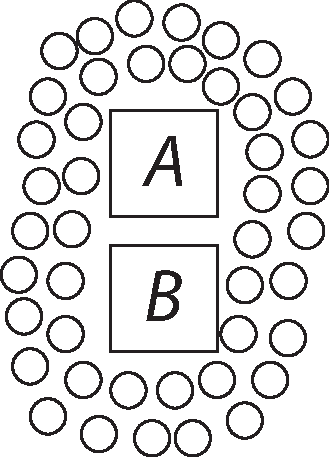
\includegraphics[trim = 0mm -3mm -5mm 0mm, clip, width=0.15\textwidth]{images/LBr719a_3-4_d1.pdf}\\
\noindent \centering\edtext{\lbrack\textit{Fig. 1}\rbrack}{\lemma{\hspace*{1,7mm}\lbrack\textit{Fig. 1}\rbrack}\killnumber\Cfootnote{Ähnliche Abbildung a.a.O.\cite{01016}, Bd.~I, S.~23.}}\\
\end{wrapfigure}
\noindent%
Mais les parties de l'air estant aussi encor grossieres; il faut les elever assez pour donner entr\'{e}e \`{a} l'air, il
\edtext{faut que}{\lemma{faut}\Bfootnote{\textit{(1)} qu'elles \textit{(2)} que \textit{L}}}
les deux corps
\edtext{$A$ $B$}{\lemma{$A$ $B$}\Bfootnote{\textit{erg. L}}}
soient autant separ\'{e}s qu'il faut pour donner entr\'{e}e \`{a} l'air i.~s.~s.
Sans cela la rupture ne s'ensuivra pas mais le corps aura ressort\protect\index{Sachverzeichnis}{ressort} c'est \`{a} dire il retournera dans la premi\`{e}re figure.%
\edlabel{LBr719a_2b}%
\newline%
Experience\protect\index{Sachverzeichnis}{experience}\edlabel{LBr719a_3a}%
\edtext{}{{\xxref{LBr719a_3a}{LBr719a_3b}}\lemma{Experience [...] deux}\Cfootnote{Vgl. a.a.O.\cite{01016}, Bd.~I, S.~25f.}}
qui le confirme pour separer deux corps polis en du Mercure,\protect\index{Sachverzeichnis}{mercure}
il suffit que ces corps soient moins polis que dans l'air, \`{a} cause que le Mercure\protect\index{Sachverzeichnis}{mercure}
est plus grossier que l'air. La partie grossiere de l'air même a ressort\protect\index{Sachverzeichnis}{ressort}, \`{a} cause de la partie subtile de l'air, qui par sa pesanteur\protect\index{Sachverzeichnis}{pesanteur} tache de se mettre entre deux.%
\edlabel{LBr719a_3b}%
\pend%
\pstart%
\textso{Corps mols, }\edlabel{LBr719a_4a}%
\edtext{}{{\xxref{LBr719a_4a}{LBr719a_4b}}\lemma{\textso{Corps}
 [...] corroy\'{e}es.}\Cfootnote{Vgl. a.a.O.\cite{01016}, Bd.~I, S.~33-35.}}%
joints par peu de faces plattes.
Il y a peut estre cent fois plus de surfaces plattes dans un grain de poudre\protect\index{Sachverzeichnis}{poudre} de diamant, que dans une grosse pi\`{e}re de taille.%
\pend%
\count\Bfootins=1200
\count\Cfootins=1200
%\newpage%
\pstart%
Dans les corps \textso{visceux} et \textso{friables} il y
\edtext{a compositions}{\lemma{a}\Bfootnote{\textit{(1)} un melange \textit{(2)} compositions \textit{L}}}
des corpuscules\protect\index{Sachverzeichnis}{corpuscule}
dont les faces sont appliqu\'{e}es immediatement, et d'autres en elles ne le sont qu'en tres peu d'endroits. Dans le visqueux ils sont parfaitement meslez, et ainsi ils sont par tous ductiles, dans l'estant \textso{coherent} par les parties dont les faces sont appliquees, et ductiles par les parties qui ont peu de faces; dans les friables les deux diff\'{e}rentes parties n'estant pas bien mesl\'{e}es, se rompent aisement. Les chauses friables deviennent visceuses, estant paistries et corroy\'{e}es.%
\edlabel{LBr719a_4b}%
\pend%
%%%%% 13.8.
\pstart%
La\edlabel{LBr719a_5a}%
\edtext{}{{\xxref{LBr719a_5a}{LBr719a_5b}}\lemma{La forge [...] davantage}\Cfootnote{Vgl. a.a.O.\cite{01016}, Bd.~I, S.~35-37.}}
forge\protect\index{Sachverzeichnis}{forge} et l'ecrouissement endurcissent
\edtext{les metaux,}{\lemma{les}\Bfootnote{\textit{(1)} corps \textit{(2)} metaux, \textit{L}}}
comme le feu\protect\index{Sachverzeichnis}{feu}, le cuivre,\protect\index{Sachverzeichnis}{cuivre} l'argent\protect\index{Sachverzeichnis}{argent}, l'or parce qu'une forte compression\protect\index{Sachverzeichnis}{compression} fait appliquer les unes aux autres en plus grand nombre: et dans ceux que la
\edtext{fonte rend}{\lemma{fonte}\Bfootnote{\textit{(1)} endurcit, comme le \textit{(2)} rend \textit{L}}}
plus fermes, comme le plomb\protect\index{Sachverzeichnis}{plomb}, l'etain\protect\index{Sachverzeichnis}{etain} etc. parce que la fluidit\'{e} de la fonte donne la libert\'{e} aux parties de s'appliquer. Les corps qui s'ammollissent et perdent leur ressort\protect\index{Sachverzeichnis}{ressort} de \protect\index{Sachverzeichnis}{dureté}duret\'{e} par le froissement\protect\index{Sachverzeichnis}{froissement} et le corroyement\protect\index{Sachverzeichnis}{corroyement} comme le cuir\protect\index{Sachverzeichnis}{cuir}, la cire\protect\index{Sachverzeichnis}{cire}, la terre\protect\index{Sachverzeichnis}{terre} grosse, l'etain\protect\index{Sachverzeichnis}{etain}, le \protect\index{Sachverzeichnis}{plomb}plomb, ont une grande
\edtext{[partie]}{\lemma{parties}\Bfootnote{\textit{L \"{a}ndert Hrsg.}}}
des parties fluides remferm\'{e}es dans des intervalles spongieux, qui lors qu'on les corroye
\edtext{se meslent}{\lemma{se}\Bfootnote{\textit{(1)} separent \textit{(2)} meslent \textit{L}}}
par tout \`{a} cause du corroyement\protect\index{Sachverzeichnis}{corroyement} qui separe les parties dont les faces estant appliqu\'{e}es les unes aux autres avant qu'on les eust froiss\'{e}e par le corroyement\protect\index{Sachverzeichnis}{corroyement} faisoient quelque connexion au lieu qu'\`{a} present ces parties qui ont peu de faces interpos\'{e}es empechent les autres de se bien joindre.
Mais les corps destitués de ces parties fluides, sont endurcis par le froissement,\protect\index{Sachverzeichnis}{froissement}
qui ne fait que les joindre davantage[:]\edlabel{LBr719a_5b}
%
\edlabel{LBr719a_6a}le bois sec
\edtext{}{{\xxref{LBr719a_6a}{LBr719a_6b}}\lemma{le bois [...] encor}\Cfootnote{Vgl. a.a.O.\cite{01016}, Bd.~I, S.~37-39.}}%
\edtext{plus dur}{\lemma{plus}\Bfootnote{\textit{(1)} humide \textit{(2)} dur \textit{L}}}
\`{a} cause de l'evaporation\protect\index{Sachverzeichnis}{evaporation} de l'humide. Le fer\protect\index{Sachverzeichnis}{fer} chaud ne fait point de
%
[3~v\textsuperscript{o}]
%
ressort\protect\index{Sachverzeichnis}{ressort} \`{a} cause des parties fluides et glissantes que le feu\protect\index{Sachverzeichnis}{feu} a introduit. Refroidi \`{a} loisir il a peu de ressort\protect\index{Sachverzeichnis}{ressort} car quelque chose de la mollesse qu'il avoit estant chaud luy demeure, lorsqu'en refroidissant les parties les plus liquides s'envolant des semblables prennent tousjours leur places, quoyque un peu moins liquides.
\pend%
\pstart%
Le fer\protect\index{Sachverzeichnis}{fer} s'endurcit estant battu \`{a} froid les corps liquides et glissans estant chassez \`{a} coups de marteau\protect\index{Sachverzeichnis}{eau}.\protect\index{Sachverzeichnis}{marteau}
\pend%
\pstart%
Le fer\protect\index{Sachverzeichnis}{fer} s'endurcit par la trempe\protect\index{Sachverzeichnis}{trempe}; fer\protect\index{Sachverzeichnis}{fer} chaud gonfl\'{e}; la partie subtile d'air recommence son effect aussitost que le feu\protect\index{Sachverzeichnis}{feu} cesse d'agir, mais elle le produit plus parfaitement sur le fer\protect\index{Sachverzeichnis}{fer} rougi, \`{a} cause de la facilit\'{e} que le feu\protect\index{Sachverzeichnis}{feu} donne aux parties du fer\protect\index{Sachverzeichnis}{fer}, de s'appliquer.
\pend%
\newpage%
\pstart%
Le fer\protect\index{Sachverzeichnis}{fer} gonfle par la trempe\protect\index{Sachverzeichnis}{trempe}: experience\protect\index{Sachverzeichnis}{experience}[,] une partie d'un fil de fer\protect\index{Sachverzeichnis}{fer} tremp\'{e}e, n'entre plus dans le trou de la filiere\protect\index{Sachverzeichnis}{filiere}, o\`{u} l'autre entre encor.%
\edlabel{LBr719a_6b}%
\pend %
\pstart%
Les\edlabel{LBr719a_7a}
\edtext{}{{\xxref{LBr719a_7a}{LBr719a_7b}}\lemma{Les ouvriers [...] refroidies}\Cfootnote{Vgl. a.a.O.\cite{01016}, Bd.~I, S.~40.}}%
ouvriers qui veuillent que l'acier\protect\index{Sachverzeichnis}{acier} rougi ne s'endurcisse pas en
\edtext{[se]}{\lemma{ce}\Bfootnote{\textit{L \"{a}ndert Hrsg.}}}
refroidissant, font ce qu'ils appellent recuire[,] le laissent dans les charbons tout une nuit, jusqu'\`{a} ce qu'ils soient \'{e}teints et même les cendres refroidies.%
\edlabel{LBr719a_7b}%
\pend%
\pstart%
Corps\edlabel{LBr719a_8a}
\edtext{}{{\xxref{LBr719a_8a}{LBr719a_8b}}\lemma{Corps [...] place}\Cfootnote{Vgl. a.a.O.\cite{01016}, Bd.~I, S.~41.}}%
souffrent generalement evaporation\protect\index{Sachverzeichnis}{evaporation} d’une partie la plus subtile et la plus
\edtext{soluble comme}{\lemma{soluble}\Bfootnote{\textit{(1)} dans l’air est compos\'{e} \textit{(2)} comme \textit{L}}} celle dont l’air grossier et
\edtext{compos\'{e}. Le}{\lemma{compos\'{e}.}\Bfootnote{\textit{(1)} Les \textit{(2)} Le \textit{L}}} flux continuel de ces parties, rend les corps liquides, et les empeche de s’appliquer par
\edtext{[leurs]}{\lemma{leur}\Bfootnote{\textit{L \"{a}ndert Hrsg.}}} surfaces plattes.
Les liqueurs\protect\index{Sachverzeichnis}{liqueur}
\edtext{[s']}{\lemma{s'}\Bfootnote{\textit{erg. Hrsg.}}}%
enflent en gla\c{c}ant comme l’acier\protect\index{Sachverzeichnis}{acier} dans la trempe\protect\index{Sachverzeichnis}{trempe}, car au premier instant que le corps liquide est reserr\'{e} au
\edtext{dehors, les parties}{\lemma{dehors,}\Bfootnote{\textit{(1)} ce qui est au dedans. \textit{(2)} les parties \textit{L}}} subtiles qui sont au dedans et qui tachent de sortir sont reflechies sur elles mêmes, ce qui leur donne un nouveau mouvement qui pousse les parties grossieres de l'eau\protect\index{Sachverzeichnis}{eau} qui ne sont pas encor appliqu\'{e}es les unes aux autres, et change leur situation; ainsi qu'il arrive dans la rarefaction\protect\index{Sachverzeichnis}{rarefaction} qui leur fait occuper plus de place.%
\edlabel{LBr719a_8b}%
\pend%
\pstart%
Par\edlabel{LBr719a_9a}
\edtext{}{{\xxref{LBr719a_9a}{LBr719a_9b}}\lemma{Par la [...] l'eau}\Cfootnote{Vgl. a.a.O.\cite{01016}, Bd.~I, S.~57.}}%
la m\^{e}me raison le soleil\protect\index{Sachverzeichnis}{soleil} endurcit la terre\protect\index{Sachverzeichnis}{terre}. Car la terre\protect\index{Sachverzeichnis}{terre} abbreuu\'{e}e d'eau\protect\index{Sachverzeichnis}{eau} unit les parties, lesquelles sont encor plus fortement unies lors que l'eau\protect\index{Sachverzeichnis}{eau} qui empechoit une plus parfaite union (comme elle avoit fait une mediocre) evapore. Par la même raison le feu\protect\index{Sachverzeichnis}{feu} endurcit la bricque ou terre\protect\index{Sachverzeichnis}{terre} cuite, parce que les parties du feu\protect\index{Sachverzeichnis}{feu} y
\edtext{[entrent]}{\lemma{entre}\Bfootnote{\textit{L \"{a}ndert Hrsg.}}}
\edtext{et [se]}{\lemma{et}\Bfootnote{\textit{(1)} unissent les parties \textit{(2)} ce \textit{L \"{a}ndert Hrsg.}}}
rendant fluides les parties leur donnent moyen de s'unir, et d'appliquer
\edtext{[leurs]}{\lemma{leur}\Bfootnote{\textit{L \"{a}ndert Hrsg.}}}
surfaces: et cette union des briques est si forte et les pores si prochaines que l'eau\protect\index{Sachverzeichnis}{eau} n'y passe plus estant trop grossiere, ainsi elle ne les detrempe\protect\index{Sachverzeichnis}{trempe} plus.
À cause que la dissolution par le feu\protect\index{Sachverzeichnis}{feu}, est plus parfaite que celle qui se fait par l'eau\protect\index{Sachverzeichnis}{eau}.%
\edlabel{LBr719a_9b}%
\pend%
\pstart%
Les\edlabel{LBr719a_10a}
\edtext{}{{\xxref{LBr719a_10a}{LBr719a_10b}}\lemma{Les cailloux [...] pores}\Cfootnote{Vgl. a.a.O., % C. \textsc{Perrault}, \cite{01016}\title{Essais de physique}, Paris 1680,
Bd.~I, S.~59-62.}}%
cailloux\protect\index{Sachverzeichnis}{caillou} marbres\protect\index{Sachverzeichnis}{marbre} pierres precieuses endurcissent par une mani\`{e}re differente. \`{A} cause des parties subtiles qui viennent par l'evaporation\protect\index{Sachverzeichnis}{evaporation} des entrailles de la terre\protect\index{Sachverzeichnis}{terre}, et rencontrent des porosit\'{e}s\protect\index{Sachverzeichnis}{porosité} bien dispos\'{e}es aux quelles elles peuuent bien unir
\edtext{[leurs]}{\lemma{leur}\Bfootnote{\textit{L \"{a}ndert Hrsg.}}}
faces.
Ces porosit\'{e}s\protect\index{Sachverzeichnis}{porosité} auparavant faisoient que cette terre\protect\index{Sachverzeichnis}{terre} estoit molle, et par le remplissement elle a est\'{e} endurcie; la maniere dont l'estain\protect\index{Sachverzeichnis}{etain} et le cuiure\protect\index{Sachverzeichnis}{cuivre} fondus ensemble s'endurcissent faisant une composition beaucoup plus dure, explique encore cet endurcissement\protect\index{Sachverzeichnis}{endurcissement}; caus\'{e} par l'introduction d'une nouvelle substance comme l'endurcissement\protect\index{Sachverzeichnis}{endurcissement} d'une matiere de cuiure\protect\index{Sachverzeichnis}{cuivre} et \'{e}tain\protect\index{Sachverzeichnis}{etain} fondus \edtext{ensembles. Aristote\protect\index{Namensregister}{\textso{Aristoteles}, 384-322 v. Chr.}%
}{\lemma{}\Bfootnote{ensembles. \textbar\ + \textit{streicht Hrsg.} \textbar\ Aristote\ \textit{L}}}
(+~\textit{\edtext{De generatione}{\lemma{De generatione}\Cfootnote{\cite{01052}\textsc{Aristoteles}, \title{De generatione animalium} II 10, 448b3, zitiert hierfür Empedokles.}}}
o\`{u} il rend raison de la sterilit\'{e} des
\edtext{mules~\phantom(\hspace{-1.2mm}+) dit}{\lemma{mules}\Bfootnote{\textit{(1)} pretendant que leur \textit{(2)} \phantom(\hspace{-1.2mm}+) dit \textit{L}}} que l'etain\protect\index{Sachverzeichnis}{etain} penetre les pores du cuiure\protect\index{Sachverzeichnis}{cuivre} et les remplit. Effectivement l'etain\protect\index{Sachverzeichnis}{etain} s'allie aisement avec tous les metaux, (+~une goutte\protect\index{Sachverzeichnis}{goutte} d'\'{e}tain\protect\index{Sachverzeichnis}{etain}
\edtext{[fondue]}{\lemma{fondu}\Bfootnote{\textit{L \"{a}ndert Hrsg.}}}
avec l'argent\protect\index{Sachverzeichnis}{argent}~+).
Trois boules 1. d'estain\protect\index{Sachverzeichnis}{etain}, l'autre de cuiure\protect\index{Sachverzeichnis}{cuivre}, troisieme d'estaint\protect\index{Sachverzeichnis}{etain} avec du cuiure\protect\index{Sachverzeichnis}{cuivre}; ces trois boules estant de même volume et pes\'{e}es on a trouu\'{e} que la boule de metail compos\'{e} pesoit presque autant que les deux autres ensemble (+~boule compos\'{e}e p\`{e}se plus d'un quart plus que celle de cuiure\protect\index{Sachverzeichnis}{cuivre} seule~+) odeur du cuiure\protect\index{Sachverzeichnis}{cuivre} et de l'estaint\protect\index{Sachverzeichnis}{etain} sans comparaison plus forte que celle des autres metaux \`{a} cause d'une matiere sulphur\'{e}e qui remplit les pores.%
\edlabel{LBr719a_10b}%
\pend%
\pstart%
La \protect\index{Sachverzeichnis}{coagulation}coagulation\edlabel{LBr719a_11a}
\edtext{}{{\xxref{LBr719a_11a}{LBr719a_11b}}\lemma{La coagulation [...] mobiles}\Cfootnote{Vgl. C. \textsc{Perrault}, \cite{01016}\title{Essais de physique}, Paris 1680, % a.a.O.\cite{01016}, 
Bd.~I, S.~62-64.}}%
et l'endurcissement\protect\index{Sachverzeichnis}{endurcissement} de la chaux\protect\index{Sachverzeichnis}{chaux} du plastre\protect\index{Sachverzeichnis}{plastre}. Chaux\protect\index{Sachverzeichnis}{chaux} forte par la violence du feu\protect\index{Sachverzeichnis}{feu}, a perdu les sels\protect\index{Sachverzeichnis}{sel} volatils et sulphur\'{e}s qui la rendoient dure; et n'ayant gueres retenu que les fixes que le feu\protect\index{Sachverzeichnis}{feu} n'emporte point mais que l'eau\protect\index{Sachverzeichnis}{eau} peut remuer; il arrive que lors que l'on \'{e}teint la chaux\protect\index{Sachverzeichnis}{chaux} l'eau \protect\index{Sachverzeichnis}{eau}excite un tel mouuement dans les differens sels\protect\index{Sachverzeichnis}{sel}, qui sont rest\'{e}s dans la chaux\protect\index{Sachverzeichnis}{chaux} et que le feu\protect\index{Sachverzeichnis}{feu} a d\'{e}tachez, qu'il s'en produit une chaleur\protect\index{Sachverzeichnis}{chaleur}, la quelle agissant sur les petites cailloux\protect\index{Sachverzeichnis}{caillou} dont le sable est compos\'{e} on fait sortir d'autres sels\protect\index{Sachverzeichnis}{sel} volatils de la même maniere que ceux que le feu\protect\index{Sachverzeichnis}{feu} avoit
\edtext{chassez hors}{\lemma{chassez}\Bfootnote{\textit{(1)} de \textit{(2)} hors \textit{L}}} la chaux\protect\index{Sachverzeichnis}{chaux}; et ces sels\protect\index{Sachverzeichnis}{sel} entrans dans la chaux\protect\index{Sachverzeichnis}{chaux} et reprenant la place de ceux qu'elle avoit perdus, luy rendent la \protect\index{Sachverzeichnis}{dureté}duret\'{e}
%
[4~r\textsuperscript{o}]
%
par une introduction de parties subtiles et formées avec des faces tres plattes,
et ainsi la \protect\index{Sachverzeichnis}{dureté}duret\'{e} est produite dans le mortier\protect\index{Sachverzeichnis}{mortier} de la
\edtext{[manière]}{\lemma{matiere}\Bfootnote{\textit{L \"{a}ndert Hrsg.}}}
que dans les \protect\index{Sachverzeichnis}{marbre}marbres:
et l'eau l'aide, en rendant les parties de la chaux\protect\index{Sachverzeichnis}{chaux} plus mobiles.%
\edlabel{LBr719a_11b}%
\pend%
\pstart%
Le \protect\index{Sachverzeichnis}{plastre}plastre\edlabel{LBr719a_12a}
\edtext{}{{\xxref{LBr719a_12a}{LBr719a_12b}}\lemma{Le plastre [...] chaux}\Cfootnote{Vgl. a.a.O.\cite{01016}, Bd.~I, S.~64.}}%
se fait d'une terre\protect\index{Sachverzeichnis}{terre} qui n'est qu'\`{a}
demi cuite et a des parties qui ont rapport \`{a} la chaux\protect\index{Sachverzeichnis}{chaux} s\c{c}avoir celles qui sont parfaitement
cuites et d'autres qui ont rapport au sable s\c{c}avoir celles qui sont demeur\'{e}es crues,
ainsi le plastre\protect\index{Sachverzeichnis}{plastre} estant reduit en poudre\protect\index{Sachverzeichnis}{poudre}
et detrempe les parties calcin\'{e}es s'\'{e}chauffant font sortir les sels\protect\index{Sachverzeichnis}{sel}
volatils dont les parties crues sont encor remplies, et causent une coagulation\protect\index{Sachverzeichnis}{coagulation}
qui n'est differente de celle du mortier\protect\index{Sachverzeichnis}{mortier} qu'en ce qu'elle est beaucoup plus promte, peutestre parce
\edtext{que les sels\protect\index{Sachverzeichnis}{sel} volatils qui sont rest\'{e}s}{\lemma{que}\Bfootnote{\textit{(1)} celles qui sont rest\'{e} \textit{(2)} les sels
[...] rest\'{e}s \textit{L}}}
dans le plastre\protect\index{Sachverzeichnis}{plastre} sont de m\^{e}me espece,
au lieu que ceux du mortier\protect\index{Sachverzeichnis}{mortier}, viennent du sable different de la chaux\protect\index{Sachverzeichnis}{chaux}.%
\edlabel{LBr719a_12b}%
\pend%
\pstart%
Le \protect\index{Sachverzeichnis}{ciment}ciment\edlabel{LBr719a_13a}
\edtext{}{{\xxref{LBr719a_13a}{LBr719a_13b}}\lemma{Le ciment [...] chaux}\Cfootnote{Vgl. a.a.O.\cite{01016}, Bd.~I, S.~64f.}}%
et la poudre\protect\index{Sachverzeichnis}{poudre de pozzolane} de pozzolane
\edtext{(eau\protect\index{Sachverzeichnis}{eau puteoly} puteoly),}{\lemma{(eau puteoly)}\Bfootnote{\textit{erg. L}}}
qui comme le plastre\protect\index{Sachverzeichnis}{plastre} sont \`{a} demy calcinez l'un par le feu\protect\index{Sachverzeichnis}{feu} du fourneau\protect\index{Sachverzeichnis}{fourneau}, l'autre par
les feux\protect\index{Sachverzeichnis}{feu} sousterrains font une liaison et un corps plus dur,
estant meslez avec la \protect\index{Sachverzeichnis}{chaux}chaux,
que ne fait le sabe parce que les sels\protect\index{Sachverzeichnis}{sel} sulphurez y sont plus degagez,
et plus prests \`{a} se mesler avec les parties terrestres de la \protect\index{Sachverzeichnis}{chaux}chaux.%
\edlabel{LBr719a_13b}%
\pend%
\count\Bfootins=1000
\count\Cfootins=1000
\pstart%
Lorsqu'on\edlabel{LBr719a_14a}
\edtext{}{{\xxref{LBr719a_14a}{LBr719a_14b}}\lemma{Lorsqu'on [...] pointe}\Cfootnote{Vgl. a.a.O.\cite{01016}, Bd.~I, S.~66-68.}}%
\'{e}chauffe un endroit du verre\protect\index{Sachverzeichnis}{verre}, et qu'en suitte on le mouille, il se fend \`{a} cet endroit
par les parties fluides agit\'{e}es d'une part par le feu\protect\index{Sachverzeichnis}{feu}, et retenues de l'autre par l'eau\protect\index{Sachverzeichnis}{eau}, en sorte
que ces parties agit\'{e}es agissent plus puissamment \`{a} l'endroit mouillé qu'aux autres par les quels
une partie des corpuscules\protect\index{Sachverzeichnis}{corpuscule}
fluides agit\'{e}s s'exhale en libert\'{e} et ne fait point un effort par sa sortie
qui soit capable de casser le verre.\protect\index{Sachverzeichnis}{verre}
Mais lors que le verre\protect\index{Sachverzeichnis}{verre} fondu est jett\'{e} soudainement dans l'eau\protect\index{Sachverzeichnis}{eau} pour former
la larme\protect\index{Sachverzeichnis}{larme}, il ne se casse pas, parce que l'eau\protect\index{Sachverzeichnis}{eau} agit de toutes parts, le mouuement que le feu\protect\index{Sachverzeichnis}{feu} avoit
excit\'{e} dans les parties fluides cesse soudainement, parcequ'elles sont toutes renferm\'{e}es au dedans et que leur
mouuement venoit de ce qu'elles avoient la libert\'{e} de sortir. L'eau\protect\index{Sachverzeichnis}{eau} agissant d'abord sur la surface l'endurcit
parcequ'elle repousse, en dedans les parties fluides par l'exclusion des quelles les particules\protect\index{Sachverzeichnis}{particule} \`{a} faces plattes n'ont plus
rien qui les empeche de s'approcher et de se joindre. Et c'est ce qui fait que dans toutes les larmes\protect\index{Sachverzeichnis}{larme} de verre\protect\index{Sachverzeichnis}{verre}
qui font l'effect dont il s'agit, il y a dans leur milieu un espace qui paroist vuide,\protect\index{Sachverzeichnis}{vide}
dans lequel apparemment sont contenues les particules\protect\index{Sachverzeichnis}{particule}
fluides que l'eau\protect\index{Sachverzeichnis}{eau} a chas\'{e}es du dedans, et qui n'attendent que quelque agitation
exterieure pour faire ces admirables effects: que lors que l'on casse la larme\protect\index{Sachverzeichnis}{larme} apres qu'elle est refroidie
elle se resout en poudre\protect\index{Sachverzeichnis}{poudre}; car ces parties fluides en grande quantit\'{e} venans \`{a} estre soudainement agit\'{e}es
\edtext{[séparent]}{\lemma{separ}\Bfootnote{\textit{L \"{a}ndert Hrsg.}}}
les autres parties jointes par des surfaces plattes.
On en voit un exemple car l'effervescence\protect\index{Sachverzeichnis}{effervescence}
\edtext{de l'esprit de vitriol}{\lemma{de l'}\Bfootnote{\textit{(1)} huile\protect\index{Sachverzeichnis}{huile de vitriol} de vitriol \textit{(2)} esprit de vitriol \textit{L}}}
avec l'huile de Tartre\protect\index{Sachverzeichnis}{huile de Tartre} est plus
\edtext{forte, \`{a} proportion que}{\lemma{forte,}\Bfootnote{\textit{(1)} \`{a} mesure qu' \textit{(2)} \`{a} proportion que \textit{L}}}
l'esprit tombe dans l'huile\protect\index{Sachverzeichnis}{huile} avec plus de force.
Les larmes\protect\index{Sachverzeichnis}{larme} chauff\'{e}es ne resolvent plus en
poudre\protect\index{Sachverzeichnis}{poudre} quand on en rompt la pointe.%
\edlabel{LBr719a_14b}%
\pend%
\pstart%
Les differentes manieres d'introduire des particules\protect\index{Sachverzeichnis}{particule} fluides ou des
particules\protect\index{Sachverzeichnis}{particule} form\'{e}es avec des faces plattes produisent les \protect\index{Sachverzeichnis}{coagulation}coagulations, les congelations, les petrifications, les dissolutions, les fusions, et toutes les autres manieres differentes par les quelles les corps sont differemment amollis ou endurcis.%
\pend%
\count\Bfootins=1100
\count\Cfootins=1100
\pstart%
Cause\edlabel{LBr719a_15a}
\edtext{}{{\xxref{LBr719a_15a}{LBr719a_15b}}\lemma{Cause [...] centre}\Cfootnote{Vgl. a.a.O.\cite{01016}, Bd.~I, S.~80-89.}}%
de la pesanteur.\protect\index{Sachverzeichnis}{pesanteur} Corps ether\'{e} a mouuement \`{a} l'entour de l'axe\protect\index{Sachverzeichnis}{axe du monde} du monde, tous les corps horsmis de
cet ether\protect\index{Sachverzeichnis}{ether}
ont une repugnance\protect\index{Sachverzeichnis}{repugnance} naturelle \`{a} la rapidite; comme un vaisseau\protect\index{Sachverzeichnis}{vaisseau} ne va pas aussi
viste que le vent\protect\index{Sachverzeichnis}{vent} qui le pousse: le mouuement de l'ether\protect\index{Sachverzeichnis}{ether} \`{a} l'entour de l'axe\protect\index{Sachverzeichnis}{axe du monde} est plus
rapide vers les poles;
(+~on pourroit l'expliquer, en disant qu'il y a même quantit\'{e} de mouuement
dans chaque \protect\index{Sachverzeichnis}{tourbillance}tourbillance~+)
chaque corps pos\'{e} entre ces tourbillons\protect\index{Sachverzeichnis}{tourbillon}
est assez large pour estre frapp\'{e} par plusieurs paralleles et concentriques. $C$, $D$ concentrices. $B$ parallele, \`{a} l'equateur $A$ le tourbillon\protect\index{Sachverzeichnis}{tourbillon} $A$ va moins viste que le tourbillon\protect\index{Sachverzeichnis}{tourbillon} $B$ (+~pourroit on s'imaginer la raison, que la raison pour
\edtext{quoy le mouvement vers le pole}{\lemma{quoy}\Bfootnote{\textit{(1)} la matiere sort du pole \textit{(2)} le [...] pole \textit{ L}}} est plus viste,
parce qu'il y a moins de matiere meue, et par consequent elle est cupable de plus de
vistesse. \edtext{[\phantom(\hspace{-1.2mm}+)]}{\lemma{\phantom(\hspace{-1.2mm}+)}\Bfootnote{\textit{erg. Hrsg.}}}
\setline{7}\pend%
\vspace{0.5em}%
\pstart%
%\vspace*{1em}
\begin{minipage}[c]{0.5\textwidth}
\hspace{15mm}
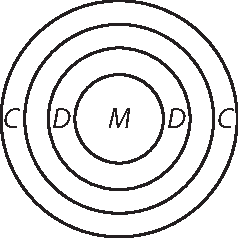
\includegraphics[width=0.4\textwidth]{images/LBr719a_3-4_d2.pdf}
\end{minipage}
\hspace{3mm}
\begin{minipage}[c]{0.5\textwidth}
%\hspace*{5mm}
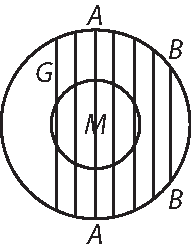
\includegraphics[width=0.35\textwidth]{images/LBr719a_3-4_d3.pdf}
\end{minipage}
\pend%
\pstart%
\vspace*{0.3em}
\hspace*{22mm}
\edtext{\lbrack\textit{Fig. 2}\rbrack}{\lemma{\hspace{1.8mm}\lbrack\textit{Fig. 2}\rbrack}\killnumber\Cfootnote{Ähnliche Abbildung a.a.O.\cite{01016}, Bd.~I, S.~84, 104.}}
\hspace*{41mm}
\edtext{\lbrack\textit{Fig. 3}\rbrack}{\lemma{\lbrack\textit{Fig. 3}\rbrack}\killnumber\Cfootnote{Ähnliche Abbildung a.a.O.\cite{01016}, Bd.~I, S.~83, 103.}}
\pend%
\vspace{0.7em}%
\pstart%
Mouuement \setline{9}du corps ether\'{e} rendu probable par le mouuement journalier de la \protect\index{Sachverzeichnis}{terre}terre;
car il est croyable que l'ether\protect\index{Sachverzeichnis}{ether} \edtext{l'emporte avec luy,}{\lemma{l'emporte avec}%
\Bfootnote{\textit{(1)} elle \textit{(2)} luy \textit{L}}}
(+~avec moins de vitesse que la sienne~+).
La matiere ether\'{e}e a ce mouuement
\edtext{naturellement, il}{\lemma{naturellement,}\Bfootnote{\textit{(1)} que \textit{(2)} il \textit{L}}}
n'accorde pas que tout ce qui est meu en rond tache de s'\'{e}loigner du centre de ce mouuement.
Et il dit qu'une boule de cire\protect\index{Sachverzeichnis}{cire} equilibrante \`{a} protect\index{Sachverzeichnis}{eau}l'eau\,
ne s'eloigne pas du centre l'eau\protect\index{Sachverzeichnis}{eau} estant agit\'{e}e en rond
\edtext{\lbrack cela}{\lemma{\lbrack cela}\Cfootnote{Eckige Klammer von Leibniz.}}
ne fait rien \`{a} l'affaire, parce que'elle n'est pas meue que par une composition de mouuement qui ne la quitte pas,
mais une boule de cire\protect\index{Sachverzeichnis}{cire} jett\'{e}e avec une fronde\protect\index{Sachverzeichnis}{fronde}
dans l'eau s'eloigneroit neanmoins du
\edtext{centre.\rbrack}{\lemma{centre.\rbrack}\Cfootnote{Eckige Klammer von Leibniz.}}
La pierre cesseroit d'estre remu\'{e}e sortant de la \protect\index{Sachverzeichnis}{fronde}fronde,
si elle n'avoit point de pesanteur,\protect\index{Sachverzeichnis}{pesanteur} \`{a} cause que les corps recoiuuent moins d'impression s'ils ont moins de pesanteur,\protect\index{Sachverzeichnis}{pesanteur} et qu'elles n'en receuuroient point,
si elle estoient sans pesanteur,\protect\index{Sachverzeichnis}{pesanteur}
\edtext{si au lieu de la boule de cire\protect\index{Sachverzeichnis}{cire}%
}{\lemma{si}\Bfootnote{\textit{(1)} l'on fait tourn \textit{(2)} au lieu [...] cire\protect\index{Sachverzeichnis}{cire} \textit{L}}} on se sert de quelque poudre\protect\index{Sachverzeichnis}{poudre} plus pesante que l'eau\protect\index{Sachverzeichnis}{eau}, et que l'on tourne sur un pivot, avec vitesse, et que le fonds soit plat
on verra que la pierre s'eloignera du centre%
\edlabel{LBr719a_15b}
%
\edtext{\lbrack+}{\lemma{\lbrack+}\Cfootnote{Eckige Klammer von Leibniz.}}~les corps plus solides recoiuuent moins de vistesse,
\edtext{mais l'ayant,}{\lemma{mais}\Bfootnote{\textit{(1)} ils \textit{(2)} l'ayant, \textit{L}}}
ils font plus d'effect ou ont plus de force, qu'un corps moins solide qui a autant de vistesse~%
\edtext{+\rbrack\ \lbrack+}{\lemma{+\rbrack\ \lbrack+}\Cfootnote{Eckige Klammern von Leibniz.}}%
~la raison que la boule de cire\protect\index{Sachverzeichnis}{cire} ne le fait pas est manifeste,
parcequ'il n'y a point de raison qui la fasse faire plus tost que l'eau\protect\index{Sachverzeichnis}{eau} qui l'environne~%
\edtext{+\rbrack\ \lbrack}{\lemma{+\rbrack\ \lbrack}\Cfootnote{Eckige Klammern von Leibniz.\hspace{20mm}}}%
il faut mieux dire que l'ether\protect\index{Sachverzeichnis}{ether} a ce mouuement, sans dire qu'il luy est naturel
%
[4 v\textsuperscript{o}]
%
pour prouuer que les corps repugnent au mouuement.%
\edtext{[\,\rbrack\,]}{\lemma{\rbrack}\Bfootnote{\textit{erg. Hrsg.}}}
\pend%
\pstart%
\protect\index{Sachverzeichnis}{experience}Experience\edlabel{LBr719a_3-4_01}\edlabel{LBr719a_16a}%
\edtext{}{{\xxref{LBr719a_16a}{LBr719a_16b}}\lemma{Experience [...] vaisseau}\Cfootnote{Vgl. a.a.O.\cite{01016}, Bd.~I, S.~93-100.}}
des balances,\protect\index{Sachverzeichnis}{balance}
on s\c{c}ait qu'elles ont un trait plus fort, \`{a} proportion qu'elles sont plus charg\'{e}es,
c'est \`{a} dire que les \protect\index{Sachverzeichnis}{balance}balances qui estant
charg\'{e}es \'{e}galement par exemple d'une livre de chaque cost\'{e}, et que l'on fait tresboucher avec dix grains ne
pourront tresboucher avec dix grains, ne pourront tresboucher avec 50 grains estant charg\'{e}es de 20 liures.
Car l'\'{e}quilibre estant dans les deux cas la pesanteur\protect\index{Sachverzeichnis}{pesanteur} ne doit point estre consider\'{e}e.
\edtext{Aristote\protect\index{Namensregister}{\textso{Aristoteles}, 384-322 v. Chr.}}{\lemma{Aristote}\Cfootnote{\cite{01002}\textit{Mech.} 10, 852a23-28.}}
croit que cela arrive \`{a} cause que le mouuement des bassins\protect\index{Sachverzeichnis}{bassin} de la balance\protect\index{Sachverzeichnis}{balance}
lorsque l'un monte l'autre descend, est oblique, et que
ce mouuement est forc\'{e} et contraire \`{a} celuy que la pesanteur\protect\index{Sachverzeichnis}{pesanteur} donne au corps qui est naturellement droit
car par exemple pour faire tresboucher le corps $A$, il faut le faire aller vers $D$, et luy faire faire le mouuement
l'oblique, $AD$, qui est contraire \`{a} son mouuement naturel qui est le mouuement droit $AC$.
Mais sans en examiner le
fondement, on n'a qu'\`{a} faire une autre balance\protect\index{Sachverzeichnis}{balance}
o\`{u} les bassins\protect\index{Sachverzeichnis}{bassin} montent tousjours en droite ligne comme cellecy:%
%
% PR: Die Abbildung [Fig. 4] muss (wie schon jetztz) an dieser Stelle folgen, weil der Text darauf bezug nimmt.
%
\pend%
\vspace{0.7em}%
\pstart%
%%\vspace*{1em}
%\begin{minipage}[t]{0.5\textwidth}
%%\hspace*{-5mm}
\centering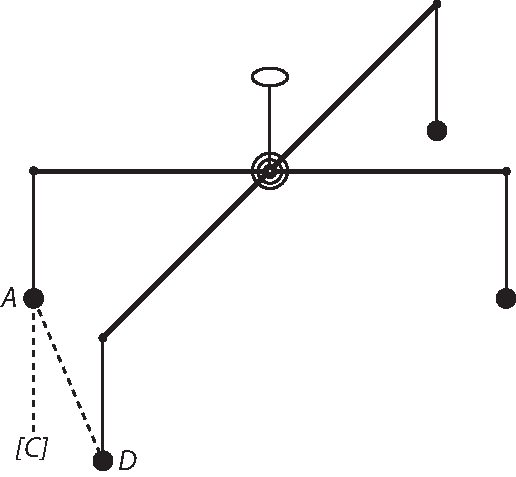
\includegraphics[width=0.45\textwidth]{images/LBr719a_3-4_d4.pdf}\\
\edtext{\lbrack\textit{Fig. 4}\rbrack}{\lemma{\lbrack\textit{Fig. 4}\rbrack}\killnumber\Cfootnote{Ähnliche Abbildung in C.~\textsc{Perrault}, \cite{01016}\title{Essais de physique}, Paris 1680, Bd.~I, S.~95.}}
% \edtext{}{\lemma{\lbrack\textit{Fig. 4}\rbrack}\killnumber\Bfootnote{C \textit{\ erg. Hrsg.}}} 
%\end{minipage}
%%\hspace*{20mm}
%\begin{minipage}[t]{0.5\textwidth}
%%\hspace*{5mm}
%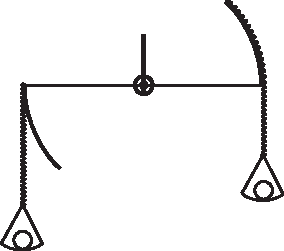
\includegraphics[width=0.7\textwidth]{images/LBr719a_3-4_d5.pdf}
%\end{minipage}
\pend%
\newpage%
\count\Bfootins=1000
\count\Cfootins=1000
\pstart%
\centering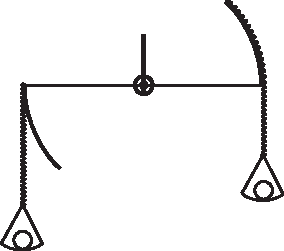
\includegraphics[width=0.27\textwidth]{images/LBr719a_3-4_d5.pdf}\\
\centering\edtext{\lbrack\textit{Fig. 5}\rbrack}{\lemma{\hspace{1.8mm}\lbrack\textit{Fig. 5}\rbrack}\killnumber\Cfootnote{Ähnliche Abbildung a.a.O.\cite{01016}, Bd.~I, S.~96.}}
\pend%
\vspace{1em}%
%\pstart
%\hspace*{15mm}
%\edtext{\lbrack\textit{Fig. 4}\rbrack}{\lemma{\lbrack\textit{Fig. 4}\rbrack}\killnumber\Cfootnote{Ähnliche Abbildung a.a.O.\cite{01016}, Bd.~I, S.~95.}}
%\edtext{}{\lemma{\lbrack\textit{Fig. 4}\rbrack}\killnumber\Bfootnote{ C \textit{\ erg. Hrsg.}}} 
%\hspace*{40mm}
%\edtext{\lbrack\textit{Fig. 5}\rbrack}{\lemma{\lbrack\textit{Fig. 5}\rbrack}\killnumber\Cfootnote{Ähnliche Abbildung a.a.O.\cite{01016}, Bd.~I, S.~96.}}
%\pend
%\vspace*{1em}
\pstart%
Quelques \setline{1}uns attribuent la force du trait au frottement\protect\index{Sachverzeichnis}{frottement} du piuot de la balance,\protect\index{Sachverzeichnis}{balance}
qui resiste au mouuement \`{a} proportion que'elle est plus charg\'{e}e. Pour refuter cecy j'ay fait une nouuelle maniere de
\edtext{balance,\protect\index{Sachverzeichnis}{balance}
prise}{\lemma{balance,\protect\index{Sachverzeichnis}{balance}}\Bfootnote{\textit{(1)} inser\'{e}e dans \textit{(2)} prise \textit{L}}}
de la construction de la machine\protect\index{Sachverzeichnis}{machine} \`{a} elever les fardeaux que j'ay propos\'{e}e dans mes notes
\edtext{sur Vitruve,\protect\index{Namensregister}{\textso{Vitruvius} Pollio, Marcus ca. 70-10 v. Chr.}}{\lemma{sur Vitruve}\Cfootnote{\cite{01014}\textsc{Vitruvius}, \title{Les dix livres d'Architecture}, hrsg. von \textsc{C. Perrault}, Paris 1673, S.~280f. und S.~324f.}}
o\`{u} j'ay appliqu\'{e} le rouleau\protect\index{Sachverzeichnis}{rouleau} \`{a} une machine\protect\index{Sachverzeichnis}{machine} montante \`{a}
\edtext{plomb\protect\index{Sachverzeichnis}{plomb}, qui n'avoit}{\lemma{plomb,}\Bfootnote{\textit{(1)} au lieu \textit{(2)} qui n'avoit \textit{L}}} est\'{e} employ\'{e} qu'\`{a} celles qui roulent sur des plans orizontaux ou peu inclinez.
\pend
\vspace{0.7em}
\pstart
\centering
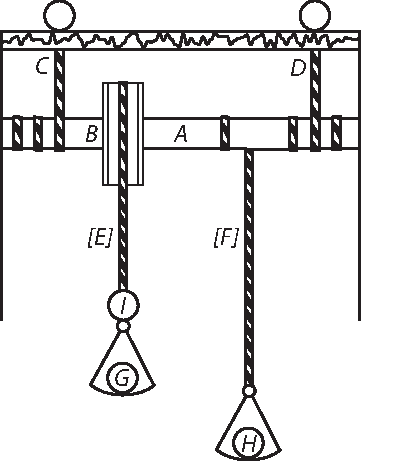
\includegraphics[width=0.44\textwidth]{images/LBr719a_3-4_d6.pdf}\\
%\noindent 
\centering
\edtext{\lbrack\textit{Fig. 6}\rbrack}{\lemma{\lbrack\textit{Fig. 6}\rbrack}\killnumber\Cfootnote{Ähnliche Abbildung in C.~\textsc{Perrault}, \cite{01016}\title{Essais de physique}, Paris 1680, Bd.~I, S.~99.}}% \edtext{}{\lemma{\lbrack\textit{Fig. 6}\rbrack}\killnumber\Bfootnote{\textit{E \ erg. Hrsg.}\quad \textit{F \ erg. Hrsg.}}}
\pend
\newpage
\pstart
Cette balance\protect\index{Sachverzeichnis}{balance}
a un rouleau,\protect\index{Sachverzeichnis}{rouleau}
par exemple qui enfile une poulie\protect\index{Sachverzeichnis}{poulie} $B$, de trois pouces de diametre.
Ces deux bouts de rouleau\protect\index{Sachverzeichnis}{rouleau}
sont soutenus par des rubans\protect\index{Sachverzeichnis}{ruban} $C$, $D$. Il y a deux autres rubans\protect\index{Sachverzeichnis}{ruban} qui
suspendent les bassins\protect\index{Sachverzeichnis}{bassin} l'un $E$ attach\'{e} \`{a} la poulie\protect\index{Sachverzeichnis}{poulie} l'autre $F$ attach\'{e} au rouleau\protect\index{Sachverzeichnis}{rouleau}
lors que le bassin\protect\index{Sachverzeichnis}{bassin} $G$ descend, et fait tourner la partie $B$, et le rouleau\protect\index{Sachverzeichnis}{rouleau}
$A$, qui fait monter le bassin\protect\index{Sachverzeichnis}{bassin} $H$, parceque les rubans\protect\index{Sachverzeichnis}{ruban} qui les soutiennent estant entortill\'{e}s d'un sens contraire l'un \`{a} l'autre. Il faut que l'un descende quand l'autre monte, il arrive aussi par
la m\^{e}me raison que lors que le bassin\protect\index{Sachverzeichnis}{bassin} $G$ descend, il fait monter et la poulie\protect\index{Sachverzeichnis}{poulie} et le rouleau\protect\index{Sachverzeichnis}{rouleau}
par le moyen des rubans\protect\index{Sachverzeichnis}{ruban} $C$ et $D$
qui sont entortill\'{e}s d'un autre sens et cette elevation du rouleau\protect\index{Sachverzeichnis}{rouleau}
et de la poulie\protect\index{Sachverzeichnis}{poulie} fait que la mont\'{e}e du bassin\protect\index{Sachverzeichnis}{bassin} $H$ est \'{e}gale \`{a} la
descente du bassin\protect\index{Sachverzeichnis}{bassin} $G$ quoyque l'entortillement\protect\index{Sachverzeichnis}{entortillement} des rubans\protect\index{Sachverzeichnis}{ruban} ne soit pas \'{e}gal, le ruban\protect\index{Sachverzeichnis}{ruban} $E$ estant
entortill\'{e} sur une grande poulie\protect\index{Sachverzeichnis}{poulie} et le ruban\protect\index{Sachverzeichnis}{ruban} $F$ sur une petite. La raison de cette egalit\'{e}
vient de ce que la grande poulie\protect\index{Sachverzeichnis}{poulie} ne laisse pas plus descendre de rubans\protect\index{Sachverzeichnis}{ruban} en tournant, que le
rouleau\protect\index{Sachverzeichnis}{rouleau}
n'en fait monter, \`{a} cause qu'en m\^{e}me temps qu'elle tourne pour laisser descendre le bassin\protect\index{Sachverzeichnis}{bassin} $G$ l'entortillement\protect\index{Sachverzeichnis}{entortillement} contraire des rubans\protect\index{Sachverzeichnis}{ruban} $C$ et $D$ fait monter toute la machine\protect\index{Sachverzeichnis}{machine}
et deminue la descente du bassin\protect\index{Sachverzeichnis}{bassin} $G$ et cette m\^{e}me elevation augmente la mont\'{e}e du bassin\protect\index{Sachverzeichnis}{bassin} $H$ et suppl\'{e}e ce qui manque au rouleau\protect\index{Sachverzeichnis}{rouleau}
qui luy sert de poulie\protect\index{Sachverzeichnis}{poulie} et qui est plus petit de deux tiers de la grande poulie\protect\index{Sachverzeichnis}{poulie}. Le poids
$I$ qui est \'{e}gal \`{a} la pesanteur\protect\index{Sachverzeichnis}{pesanteur} du rouleau\protect\index{Sachverzeichnis}{rouleau}
et de la grande poulie\protect\index{Sachverzeichnis}{poulie} est adjout\'{e} au bassin\protect\index{Sachverzeichnis}{bassin} $G$ \`{a} fin de
mettre la balance\protect\index{Sachverzeichnis}{balance}
en equilibre. Or il est evident que le mouuement de cette balance\protect\index{Sachverzeichnis}{balance}
n'a aucun frottement\protect\index{Sachverzeichnis}{frottement}, puis,
qu'il ne s'agit que de faire plier en rond les quatre rubans\protect\index{Sachverzeichnis}{ruban} ce qui n'est que comme rien. Mais le plus
important est que cet empechement n'est jamais different, quelque poids qu'on puisse mettre dans la balance,\protect\index{Sachverzeichnis}{balance}
le pliement des rubans\protect\index{Sachverzeichnis}{ruban} n'estant pas plus difficil dans un grand que dans un petit
\edtext{poids.\edlabel{LBr719a_3-4_02}%
\newline%
\indent%
Autre experience\protect\index{Sachverzeichnis}{experience}%
}{\lemma{poids}\Bfootnote{\textit{(1)} ; la seconde \textit{(2)} . Autre experience\protect\index{Sachverzeichnis}{experience} \textit{ L}}}
pour prouuer la repugnance des corps au mouuement, s\c{c}avoir que lors qu'on fait tourner un
vaisseau\protect\index{Sachverzeichnis}{vaisseau} horizontalement sur son centre l'eau\protect\index{Sachverzeichnis}{eau} ne tourne point et il y a apparence, que cela ne se fait point par autre raison que par la repugnance que l'\edtext{[eau\protect\index{Sachverzeichnis}{eau}]}{\lemma{au}\Bfootnote{\textit{L \"{a}ndert Hrsg.}}} a au mouuement par ce qu'on ne voit point qu'il y ait
autre cause qui l'empeche de suiure le mouuement du vaisseau\protect\index{Sachverzeichnis}{vaisseau}.%
\edlabel{LBr719a_16b}%
%
%
% PR: Keine händische Nachbearbeitung der Cfootnotes mehr nötig (Stand 23.09.2015).
%
%
\pend%
\pstart%
La 3eme\edlabel{LBr719a_17a}%
\edtext{}{{\xxref{LBr719a_17a}{LBr719a_17b}}\lemma{La 3eme [...] terrestres}\Cfootnote{Vgl. a.a.O.\cite{01016}, Bd.~I, S.~100.}}
experience\protect\index{Sachverzeichnis}{experience} est celle de deux bateaux
dont le plus charg\'{e} enfonce d'avantage et donne plus de prise au courant, et neantmoins il avance moins.
\pend%
\pstart%
Supposons maintenant que les corps ont repugnance\protect\index{Sachverzeichnis}{repugnance} au mouuement, il faut supposer aussi que
le mouuement de la matiere ether\'{e}e est plus rapide vers les cotes parceque le mouuement circulaire est moins
simple et par consequent plus facile que le droit, donc il faut plus de force pour
\edtext{faire [courir]}{\lemma{faire}\Bfootnote{\textit{(1)} tourner \textit{(2)} court \textit{L \"{a}ndert Hrsg.}}} \edtext{et dans un petit}{\lemma{et dans un}\Bfootnote{\textit{(1)} grand \textit{(2)} petit \textit{L}}} cercle, 
\edtext{que dans un grand cercle}{\lemma{que dans un}\Bfootnote{\textit{(1)} petit cer \textit{(2)} grand cercle \textit{L}}} qui approche de la droite. On pourroit objecter que le mouuement aussi
est moins viste, mais il suffit de s\c{c}auoir que les corps repugnent au mouuement circulaire. Autre objection qu'il faudroit que la matiere allat plus viste
\edtext{vers proche}{\lemma{vers}\Bfootnote{\textit{(1)} les \textit{(2)} proche \textit{L}}}
du centre aussi bien que proche
\edtext{[des]}{\lemma{du}\Bfootnote{\textit{L \"{a}ndert Hrsg.}}} poles.
Cette objection, dit il seroit bien pressante,
si l'on estoit asseur\'{e} quelle est la pesanteur\protect\index{Sachverzeichnis}{pesanteur} proche du centre et m\^{e}me qu'il y a des corps pesans terrestres.%
%
\edlabel{LBr719a_17b}%
\pend%
\pstart%
\protect\index{Sachverzeichnis}{experience}Experience\edlabel{LBr719a_18a}%
\edtext{}{{\xxref{LBr719a_18a}{LBr719a_18b}}\lemma{Experience [...] s'amassent}\Cfootnote{Vgl. a.a.O.\cite{01016}, Bd.~I, S.~109f.}}
du \protect\index{Sachverzeichnis}{gouvernail}gouuernail: car la situation du gouuernail le fait trouuer plus de resistance\protect\index{Sachverzeichnis}{resistance} dans l'eau\protect\index{Sachverzeichnis}{eau}, qui l'empeche
de suiure la vistesse du vent\protect\index{Sachverzeichnis}{vent}, donc il ira du cost\'{e} qui l'empeche moins.
2\textsuperscript{de} experience,\protect\index{Sachverzeichnis}{experience} l'eau\protect\index{Sachverzeichnis}{eau} qu'on fait tourner dans un
vase\protect\index{Sachverzeichnis}{vase} rond et poli plat, par le fonds en sorte que le fonds du vase\protect\index{Sachverzeichnis}{vase} demeurant immobile l'eau\protect\index{Sachverzeichnis}{eau} ne laisse pas de tourner car
si on y jette de la sciure\protect\index{Sachverzeichnis}{sciure} de bois\protect\index{Sachverzeichnis}{bois}, on remarquera que la plus legere et qui nage ou sur la surface de l'eau\protect\index{Sachverzeichnis}{eau} ou entre
deux eaux\protect\index{Sachverzeichnis}{eau} estant emport\'{e}e sans resistance\protect\index{Sachverzeichnis}{resistance} par le cours de l'eau\protect\index{Sachverzeichnis}{eau} suit de telle sorte la direction que chaque particule\protect\index{Sachverzeichnis}{particule}
\edtext{de sciure\protect\index{Sachverzeichnis}{sciure}}{\lemma{particule de}\Bfootnote{\textit{(1)} deux eaux\protect\index{Sachverzeichnis}{eau} estant empo \textit{(2)} sciure \textit{L}}}
decrit tousjours un m\^{e}me cercle, et qu'au contraire s'il y a quelques
\edtext{parties qui}{\lemma{parties}\Bfootnote{\textit{(1)} de \textit{(2)} qui \textit{L}}}
tombent sur le fonds qui demeure immobile, et s'y attachent en sorte qu'elles resistent en quelque maniere au mouuement de \protect\index{Sachverzeichnis}{eau}l'eau, elles ne suivent point la direction circulaire, mais tournent en ligne spirale jusqu'\`{a} ce
qu'elles se rendent au milieu, o\`{u} elles s'amassent.
%
\edlabel{LBr719a_18b}%
\pend%
\pstart%
Ces deux\edlabel{LBr719a_19a}%
\edtext{}{{\xxref{LBr719a_19a}{LBr719a_19b}}\lemma{Ces deux [...] vistesse}\Cfootnote{Vgl. a.a.O.\cite{01016}, Bd.~I, S.~110f.}}
experiences\protect\index{Sachverzeichnis}{experience} prouuent comme un corps pesant va vers le centre de son plan;
troiseme experience\protect\index{Sachverzeichnis}{experience} de mettre une eau\protect\index{Sachverzeichnis}{eau} courante dans un canal:
la boule de cire\protect\index{Sachverzeichnis}{cire} d'egale
pesanteur\protect\index{Sachverzeichnis}{pesanteur} \`{a} celle de \protect\index{Sachverzeichnis}{eau}l'eau.
Quand elle nage avec l'eau\protect\index{Sachverzeichnis}{eau}
\edtext{[elle]}{\lemma{elle}\Bfootnote{\textit{erg. Hrsg.}}}
\edtext{ne va pas au fonds,}{\lemma{ne}\Bfootnote{\textit{(1)} s'enfonce pas \textit{(2)} va pas au fonds, \textit{L}}}
mais quand on la retient par un filet ou autrement, et l'empeche de couler elle ira au fonds, \`{a} cause que la surface d'en haut coule auec plus de vistesse
%
\edlabel{LBr719a_19b}
(\hspace{-1.2mm}\phantom)+~si on pouuait faire en sorte que l'eau\protect\index{Sachverzeichnis}{eau} aille plus viste en bas faisant la courir dans un canal de verre\protect\index{Sachverzeichnis}{verre} transparent plus apre en haut qu'en bas, la boule arrest\'{e}e monteroit en ce cas; et ce qui est plus pesant que l'eau\protect\index{Sachverzeichnis}{eau} car la boule pese bien autant seroit pouss\'{e} en haut, si la difference de la pesanteur\protect\index{Sachverzeichnis}{pesanteur} est petite; ou si la pesanteur\protect\index{Sachverzeichnis}{pesanteur} fait moins que la difference des mouuemens dans
\edtext{l'eau\protect\index{Sachverzeichnis}{eau}\hspace{-1.2mm}\phantom(~+)
%
si le corps\edlabel{LBr719a_20a}%
\edtext{}{{\xxref{LBr719a_20a}{LBr719a_20b}}\lemma{si le corps [...] paroist pas}\Cfootnote{Vgl. a.a.O.\cite{01016}, Bd.~I, S.~118f.}}%
}{\lemma{l'eau\hspace{-1.2mm}\phantom(~+)}\Bfootnote{\textit{(1)} les corps pesans vont aussi vers le centre de la terre\protect\index{Sachverzeichnis}{terre} en ligne (+\hspace{-1.2mm}\phantom) NB \textit{(2)} si le corps \textit{ L}}}
pesans
\edtext{descend d'un mouuvement compos\'{e}}{\lemma{descend}\Bfootnote{\textit{(1)} dans une ligne compos\'{e}e \textit{(2)} d'un mouuvement compos\'{e} \textit{L}}}
de 3, \hspace{-1.2mm}\phantom(%
1) du general de la matiere etherienne le m\^{e}me que la terre\protect\index{Sachverzeichnis}{terre}\phantom(%
2) d'un cercle \`{a} un concentrique,\phantom(%
3) d'un parallele \`{a} un autre, ligne comme spirale, mais elle ne paroist droite, \`{a} cause que le mouuement etherien ne paroist pas.%
%
\edlabel{LBr719a_20b}
%
(+~Je crois qu'elle seroit encor courbe, et par la composition des deux autres.~+)
%
Les banderoles\edlabel{LBr719a_21a}%
\edtext{}{{\xxref{LBr719a_21a}{LBr719a_21b}}\lemma{Les banderoles [...] les autres}\Cfootnote{Vgl. a.a.O.\cite{01016}, Bd.~I, S.~120.}}
des vaisseaux\protect\index{Sachverzeichnis}{vaisseau} qui sont poussez par le vent\protect\index{Sachverzeichnis}{vent} ont
\edtext{[leurs]}{\lemma{leur}\Bfootnote{\textit{L \"{a}ndert Hrsg.}}}
pointes tourn\'{e}es vers la proue, et
\edtext{[celles]}{\lemma{celle}\Bfootnote{\textit{L \"{a}ndert Hrsg.}}}
de ceux qui sont emport\'{e}s par les courans l'ont vers
la poupe, estant traisn\'{e}es par le vaisseau\protect\index{Sachverzeichnis}{vaisseau}, et
\edtext{[non]}{\lemma{n'ont}\Bfootnote{\textit{L \"{a}ndert Hrsg.}}}
pas emport\'{e}es par le vent\protect\index{Sachverzeichnis}{vent} comme les autres.
%
\edlabel{LBr719a_21b}%
\pend%
\count\Bfootins=1500
\count\Cfootins=1500
\count\Afootins=1500
%%%%  PR: Hier endet das Stück.